\section{Information Dynamics of Thinking}
\label{section:idyot}

\subsection{Information Dynamics}
\label{section:information-dynamics}

In natural language processing, n-gram models are often employed to track the frequency of chains of symbols in a given signal \citep{sproat1996stochastic}.  For instance, if examining textual data, a unigram model would count the frequency of individual words, whereas a bigram model would track the frequency of pairs of words.  It is clear that one can then utilize the information content measure on a unigram model and the conditional entropy measure on the bigram model in order to quantify the amount of information in that model (see section \ref{section:information-theory}). Extrapolating further, higher-order n-gram models would model longer sequences of symbols, which could be analyzed using longer chains of conditional entropy.  Considering a stream of symbols, one can then see that the information content and entropy of the stream will rise and fall according to the observed symbols.  This is what is meant by \textit{information dynamics}: the dynamic change in information over time and context.

\subsection{Information-Efficient Cognitive Architecture}
\label{section:information-efficient-cognitive-architecture}

The Information Dynamics of Thinking \citep{wiggins2018creativity} (IDyOT) is a cognitive architecture based on the principle that the human mind represents data according to the heuristic of information-efficiency.  That is, in its internal representations, the mind seeks to use the least amount of bits to do so.  In addition, IDyOT strives for a minimal set of processes and assumptions to describe cognitive phenomena, and yet still maintain the inherent dual quality of human memory: that representations in the mind are both learned and tied to temporal events with sequence and ordering, yet are also atemporal with regard to other situated concepts in the mind.

An example of the IDyOT memory in action is shown in Figure \ref{figure:idyot-memory} \citep{wiggins2018creativity}.  In it, we can see the two parallel memories: sequential memory in the foreground and semantic memory in the background.  These two memories are parallel in that the symbols seen in the sequential memory are tied to elements in the semantic memory such that the symbols maintain their temporal sequencing, but can be related atemporally in the semantic space.  In addition, we see the hierarchical nature of representation in the diagram.  Sequences of symbols in the sequential memory are chunked together in a subordinate layer into a single symbol in the superordinate layer.  In the parallel semantic memory, the trajectory of this sequence through a semantic space is abstracted to a single element in the superordinate layer.

\begin{figure}
  \centering
  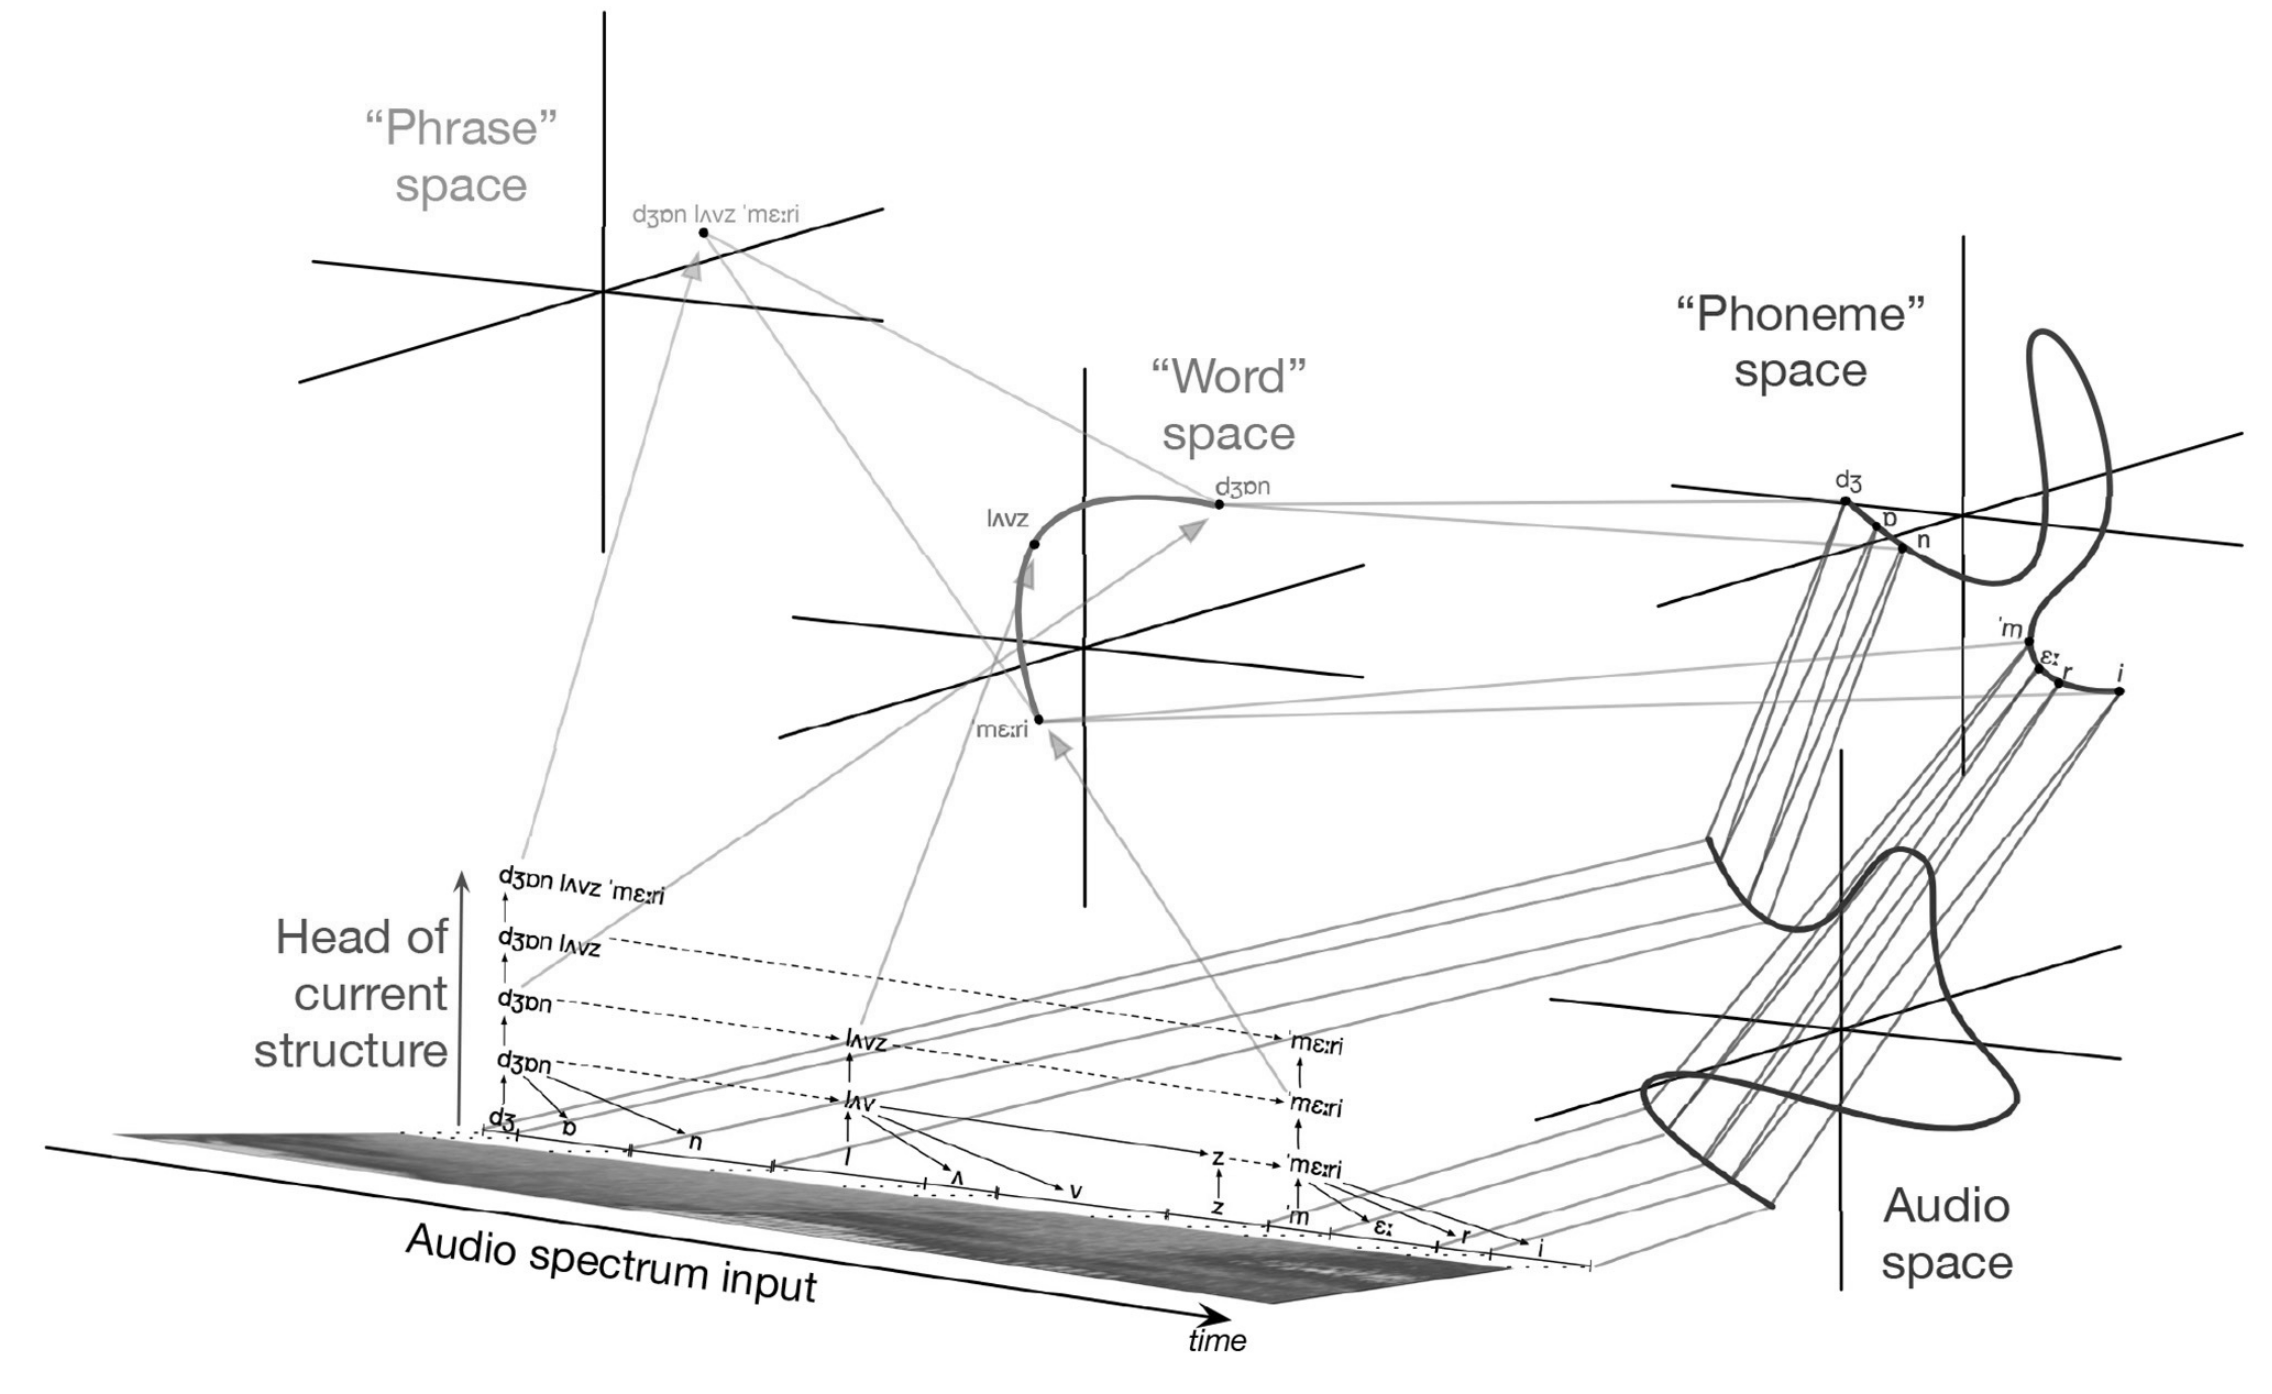
\includegraphics[width=\linewidth]{fig/idyot-memory-bw.png}
  \caption{Illustration of IDyOT memory.\\ Reproduced from (Wiggins, 2018) with the author's permission.}
  \label{figure:idyot-memory}
\end{figure}

This hierarchical representation is driven by three processes, in the same vein as the non-conconscious processors of the Global Workspace Theory \citep{baars1993cognitive}: segmentation, categorization, and abstraction.  Segmentation operates on the sequential memory by splitting the stream of observed symbols into chunks, whereas categorization operates on the semantic memory by grouping similar instances in the space into categories.  Abstraction ties these two processes together by taking the chunks formed in segmentation as trajectories of categories found in categorization, and transforming it as a single spectral representation in the superordinate abstraction layer.

\subsection{Boundary Entropy Segmentation}
\label{subsection:boundary-entropy-segmentation}

Since entropy represents the amount of uncertainty at what comes next, it makes sense that a jump in entropy would mark the beginning of a new semantic segment.  For instance, when in conversation, at the beginning of a sentence, entropy is high because the listener has little idea what the speaker will say next. As the sentence proceeds, the listener will be better able to predict what comes next, maybe even being able to finish the sentence for the speaker, meaning entropy is steadily decreasing until the end of the sentence.  Once the sentence is finished, the listener again is less sure what will come next, and so entropy rises.  Therefore, at this rise in entropy, we would make a cut, resulting in a segment naturally representing the sentence just spoken.  This method of segmenting a stream of data has been shown to be effective for cue prediction in music \citep{wiggins2010cue} and parsing language \citep{sproat1996stochastic}.

\subsection{Semantic Space Categorization}
\label{section:semantic-space-categorization}

In the Information Dynamics of Thinking, the semantic memory -- the portion of memory that represents time-invariant relationships -- is represented as a collection of conceptual spaces \citep{gardenfors2004conceptual}.  Elements in these spaces are spectral representations of trajectories of elements from less-abstract spaces \citep{chella2015cognitive}, which themselves may be spectral representations.  Being an instantiation of a conceptual space, regions in these semantic spaces correspond to properties or concepts, and so by grouping elements of the space together according to their similarity, the resulting categories correspond to the concepts of a conceptual space.

Since the IDyOT memory wants to be as information-efficient as possible in representation, the \textit{maximum entropy reduction criterion} is used to ensure that the categorization of a space is maximally information efficient \citep{quinlan1983learning}.  However, since the most efficient categorization would be a single vacuous category, the \textit{categorical convexity criterion} is used to ensure that categories are convex, for the same reasons concepts are convex in a conceptual space \citep{gardenfors2004conceptual}.

\subsection{Hierarchy Construction}
\label{section:hierarch-construction}

The hierarchical construction of abstraction layers \citep{chella2008cognitive} is performed by first taking the sequence of symbols of a chunk from the segmentation process in the sequential memory, then finding the trajectory of those symbols in the parallel semantic space.  A spectral representation of that trajectory is then found and placed in the semantic space of the superordinate abstraction layer and given a label to serve as the symbol in the parallel sequential memory at that superordinate layer.

Since all three processes of segmentation, categorization, and abstraction occur at any level of abstraction, the result is a hierarchy of increasingly abstract layers, each composed of spectral representations of segments chunked by boundary entropy from the subordinate layer.  In this manner, the higher layers are not only more semantically rich, being spectral abstractions from lower layers, but are information-efficient, being segmented and categorized according to their information-theoretic properties.









%The sequential memory in IDyOT is represented as a hierarchy of chains of symbols. As the agent perceives a continuous stream of perception from the environment, it first discretizes that stream into moments, and links those discretized percepts as symbols in an ever-growing chain.  By examining time-varying information-theoretic properties of this chain, it can be chunked into a series of segments composed of a sequence of symbols.  
%
%This segment can then be abstracted by a representative symbol in the superior layer and can be said to subsume the inferior segment.  This process is done recursively until no more abstraction can be performed.
%
%\subsection{Spectral Representations of Meaning}
%\label{subsection:spectral-representations-of-meaning}
%
%\subsection{Semantic Memory}
%\label{subsection:semantic-memory}
%
%If the sequential memory can be though of as how concepts relate to eachother over time, semantic memory can be thought of as how those concepts relate to eachother outside of time.  In IDyOT this is modeled using conceptual spaces.  At any given layer of abstraction in the sequential memory, there exists a parallel semantic space for the symbols of that layer.  This allow us to think of a segment of symbols in sequential memory as a trajectory of concepts in semantic memory.  
%
%By looking at a spectral representation of this trajectory, the time-varying properties of the segment are removed, and this spectral representation can be thought of as an abstraction of the segment, and therefore as the abstracted symbol in the superior layer of the sequential memory.
